\chapter{Strongly connectivity}

\index{strongly connected graph}

In a directed graph,
the edges can be traversed in one direction only,
so even if the graph is connected,
this does not guarantee that there would be
a path from a node to another node.
For this reason, it is meaningful to define a new concept
that requires more than connectivity.

A graph is \key{strongly connected}
if there is a path from any node to all
other nodes in the graph.
For example, in the following picture,
the left graph is strongly connected
while the right graph is not.

\begin{center}
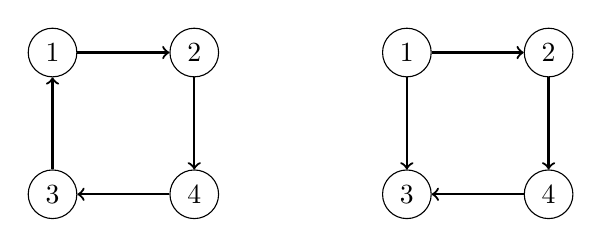
\begin{tikzpicture}[scale=0.9]
\node[draw, circle] (1) at (1,1) {$1$};
\node[draw, circle] (2) at (3,1) {$2$};
\node[draw, circle] (3) at (1,-1) {$3$};
\node[draw, circle] (4) at (3,-1) {$4$};

\path[draw,thick,->] (1) -- (2);
\path[draw,thick,->] (2) -- (4);
\path[draw,thick,->] (4) -- (3);
\path[draw,thick,->] (3) -- (1);

\node[draw, circle] (1b) at (6,1) {$1$};
\node[draw, circle] (2b) at (8,1) {$2$};
\node[draw, circle] (3b) at (6,-1) {$3$};
\node[draw, circle] (4b) at (8,-1) {$4$};

\path[draw,thick,->] (1b) -- (2b);
\path[draw,thick,->] (2b) -- (4b);
\path[draw,thick,->] (4b) -- (3b);
\path[draw,thick,->] (1b) -- (3b);
\end{tikzpicture}
\end{center}

The right graph is not strongly connected
because, for example, there is no path
from node 2 to node 1.

\index{strongly connected component}
\index{component graph}

The \key{strongly connected components}
of a graph divide the graph into strongly connected
parts that are as large as possible.
The strongly connected components form an
acyclic \key{component graph} that represents
the deep structure of the original graph.

For example, for the graph
\begin{center}
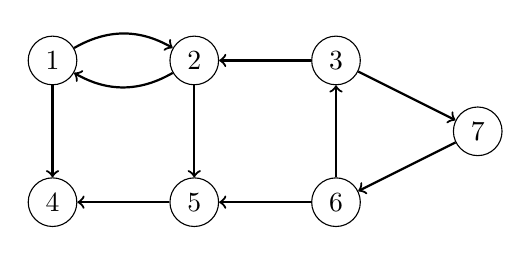
\begin{tikzpicture}[scale=0.9,label distance=-2mm]
\node[draw, circle] (1) at (-1,1) {$7$};
\node[draw, circle] (2) at (-3,2) {$3$};
\node[draw, circle] (4) at (-5,2) {$2$};
\node[draw, circle] (6) at (-7,2) {$1$};
\node[draw, circle] (3) at (-3,0) {$6$};
\node[draw, circle] (5) at (-5,0) {$5$};
\node[draw, circle] (7) at (-7,0) {$4$};

\path[draw,thick,->] (2) -- (1);
\path[draw,thick,->] (1) -- (3);
\path[draw,thick,->] (3) -- (2);
\path[draw,thick,->] (2) -- (4);
\path[draw,thick,->] (3) -- (5);
\path[draw,thick,->] (4) edge [bend left] (6);
\path[draw,thick,->] (6) edge [bend left] (4);
\path[draw,thick,->] (4) -- (5);
\path[draw,thick,->] (5) -- (7);
\path[draw,thick,->] (6) -- (7);
\end{tikzpicture}
\end{center}
the strongly connected components are as follows:
\begin{center}
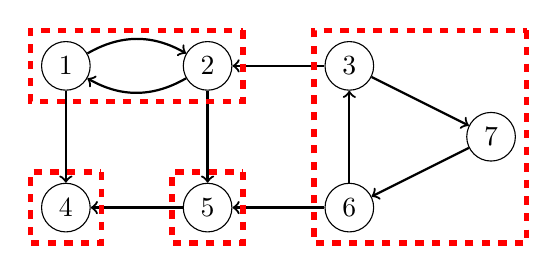
\begin{tikzpicture}[scale=0.9]
\node[draw, circle] (1) at (-1,1) {$7$};
\node[draw, circle] (2) at (-3,2) {$3$};
\node[draw, circle] (4) at (-5,2) {$2$};
\node[draw, circle] (6) at (-7,2) {$1$};
\node[draw, circle] (3) at (-3,0) {$6$};
\node[draw, circle] (5) at (-5,0) {$5$};
\node[draw, circle] (7) at (-7,0) {$4$};

\path[draw,thick,->] (2) -- (1);
\path[draw,thick,->] (1) -- (3);
\path[draw,thick,->] (3) -- (2);
\path[draw,thick,->] (2) -- (4);
\path[draw,thick,->] (3) -- (5);
\path[draw,thick,->] (4) edge [bend left] (6);
\path[draw,thick,->] (6) edge [bend left] (4);
\path[draw,thick,->] (4) -- (5);
\path[draw,thick,->] (5) -- (7);
\path[draw,thick,->] (6) -- (7);

\draw [red,thick,dashed,line width=2pt] (-0.5,2.5) rectangle (-3.5,-0.5);
\draw [red,thick,dashed,line width=2pt] (-4.5,2.5) rectangle (-7.5,1.5);
\draw [red,thick,dashed,line width=2pt] (-4.5,0.5) rectangle (-5.5,-0.5);
\draw [red,thick,dashed,line width=2pt] (-6.5,0.5) rectangle (-7.5,-0.5);
\end{tikzpicture}
\end{center}
The corresponding component graph is as follows:
\begin{center}
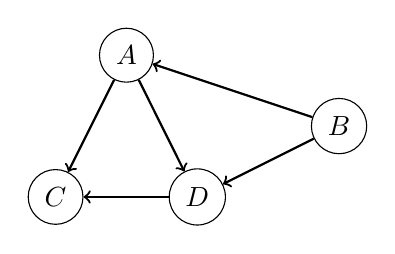
\begin{tikzpicture}[scale=0.9]
\node[draw, circle] (1) at (-3,1) {$B$};
\node[draw, circle] (2) at (-6,2) {$A$};
\node[draw, circle] (3) at (-5,0) {$D$};
\node[draw, circle] (4) at (-7,0) {$C$};

\path[draw,thick,->] (1) -- (2);
\path[draw,thick,->] (1) -- (3);
\path[draw,thick,->] (2) -- (3);
\path[draw,thick,->] (2) -- (4);
\path[draw,thick,->] (3) -- (4);
\end{tikzpicture}
\end{center}
The components are $A=\{1,2\}$,
$B=\{3,6,7\}$, $C=\{4\}$ and $D=\{5\}$.

A component graph is an acyclic, directed graph,
so it is easier to process than the original graph.
Since the graph does not contain cycles,
we can always construct a topological sort and
use dynamic programming techniques like those
presented in Chapter 16.

\section{Kosaraju's algorithm}

\index{Kosaraju's algorithm}

\key{Kosaraju's algorithm} is an efficient
method for finding the strongly connected components
of a directed graph.
The algorithm performs two depth-first searches:
the first search constructs a list of nodes
according to the structure of the graph,
and the second search forms the strongly connected components.

\subsubsection{Search 1}

The first phase of Kosaraju's algorithm constructs
a list of nodes in the order in which a
depth-first search processes them.
The algorithm goes through the nodes,
and begins a depth-first search at each 
unprocessed node.
Each node will be added to the list
after it has been processed.

In the example graph, the nodes are processed
in the following order:
\begin{center}
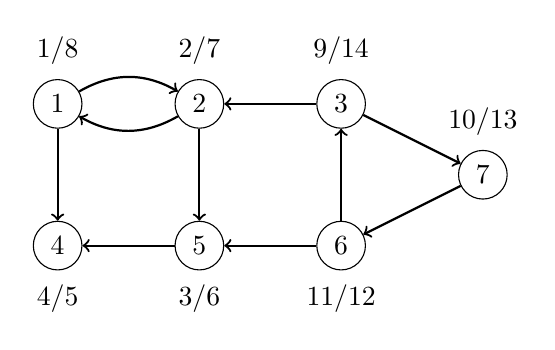
\begin{tikzpicture}[scale=0.9,label distance=-2mm]
\node[draw, circle] (1) at (-1,1) {$7$};
\node[draw, circle] (2) at (-3,2) {$3$};
\node[draw, circle] (4) at (-5,2) {$2$};
\node[draw, circle] (6) at (-7,2) {$1$};
\node[draw, circle] (3) at (-3,0) {$6$};
\node[draw, circle] (5) at (-5,0) {$5$};
\node[draw, circle] (7) at (-7,0) {$4$};

\node at (-7,2.75) {$1/8$};
\node at (-5,2.75) {$2/7$};
\node at (-3,2.75) {$9/14$};
\node at (-7,-0.75) {$4/5$};
\node at (-5,-0.75) {$3/6$};
\node at (-3,-0.75) {$11/12$};
\node at (-1,1.75) {$10/13$};

\path[draw,thick,->] (2) -- (1);
\path[draw,thick,->] (1) -- (3);
\path[draw,thick,->] (3) -- (2);
\path[draw,thick,->] (2) -- (4);
\path[draw,thick,->] (3) -- (5);
\path[draw,thick,->] (4) edge [bend left] (6);
\path[draw,thick,->] (6) edge [bend left] (4);
\path[draw,thick,->] (4) -- (5);
\path[draw,thick,->] (5) -- (7);
\path[draw,thick,->] (6) -- (7);
\end{tikzpicture}
\end{center}

The notation $x/y$ means that
processing the node started at moment $x$
and ended at moment $y$.
The following list contains the nodes
sorted according to their ending times:

\begin{tabular}{ll}
\\
node & ending time \\
\hline
4 & 5 \\
5 & 6 \\
2 & 7 \\
1 & 8 \\
6 & 12 \\
7 & 13 \\
3 & 14 \\
\\
\end{tabular}
% 
% In the second phase of the algorithm,
% the nodes will be processed
% in reverse order: $[3,7,6,1,2,5,4]$.

\subsubsection{Search 2}

The second phase of the algorithm
forms the strongly connected components
of the graph.
First, the algorithm reverses every
edge in the graph.
This makes sure that during the second search,
we will always find strongly connected
components that do not have extra nodes.

After reversing the edges,
the example graph is as follows:
\begin{center}
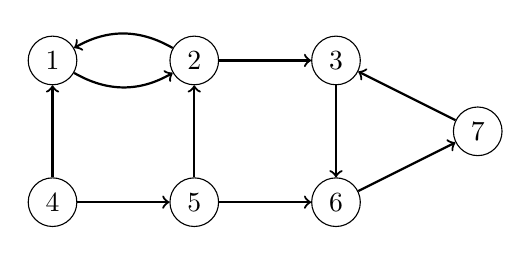
\begin{tikzpicture}[scale=0.9,label distance=-2mm]
\node[draw, circle] (1) at (-1,1) {$7$};
\node[draw, circle] (2) at (-3,2) {$3$};
\node[draw, circle] (4) at (-5,2) {$2$};
\node[draw, circle] (6) at (-7,2) {$1$};
\node[draw, circle] (3) at (-3,0) {$6$};
\node[draw, circle] (5) at (-5,0) {$5$};
\node[draw, circle] (7) at (-7,0) {$4$};

\path[draw,thick,<-] (2) -- (1);
\path[draw,thick,<-] (1) -- (3);
\path[draw,thick,<-] (3) -- (2);
\path[draw,thick,<-] (2) -- (4);
\path[draw,thick,<-] (3) -- (5);
\path[draw,thick,<-] (4) edge [bend left] (6);
\path[draw,thick,<-] (6) edge [bend left] (4);
\path[draw,thick,<-] (4) -- (5);
\path[draw,thick,<-] (5) -- (7);
\path[draw,thick,<-] (6) -- (7);
\end{tikzpicture}
\end{center}

After this, the algorithm goes through
the list of nodes created by the first search
in \emph{reverse} order.
If a node does not belong to a component,
the algorithm creates a new component
and starts a depth-first search
that adds all new nodes found during the search
to the new component.

In the example graph, the first component
begins at node 3:

\begin{center}
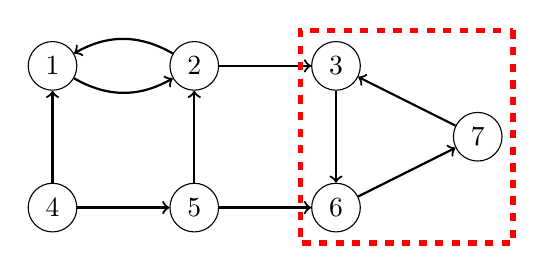
\begin{tikzpicture}[scale=0.9,label distance=-2mm]
\node[draw, circle] (1) at (-1,1) {$7$};
\node[draw, circle] (2) at (-3,2) {$3$};
\node[draw, circle] (4) at (-5,2) {$2$};
\node[draw, circle] (6) at (-7,2) {$1$};
\node[draw, circle] (3) at (-3,0) {$6$};
\node[draw, circle] (5) at (-5,0) {$5$};
\node[draw, circle] (7) at (-7,0) {$4$};

\path[draw,thick,<-] (2) -- (1);
\path[draw,thick,<-] (1) -- (3);
\path[draw,thick,<-] (3) -- (2);
\path[draw,thick,<-] (2) -- (4);
\path[draw,thick,<-] (3) -- (5);
\path[draw,thick,<-] (4) edge [bend left] (6);
\path[draw,thick,<-] (6) edge [bend left] (4);
\path[draw,thick,<-] (4) -- (5);
\path[draw,thick,<-] (5) -- (7);
\path[draw,thick,<-] (6) -- (7);

\draw [red,thick,dashed,line width=2pt] (-0.5,2.5) rectangle (-3.5,-0.5);
%\draw [red,thick,dashed,line width=2pt] (-4.5,2.5) rectangle (-7.5,1.5);
%\draw [red,thick,dashed,line width=2pt] (-4.5,0.5) rectangle (-5.5,-0.5);
%\draw [red,thick,dashed,line width=2pt] (-6.5,0.5) rectangle (-7.5,-0.5);
\end{tikzpicture}
\end{center}

Note that since all edges were reversed,
the component does not ''leak'' to other parts in the graph.

\begin{samepage}
The next nodes in the list are nodes 7 and 6,
but they already belong to a component.
The next new component begins at node 1:

\begin{center}
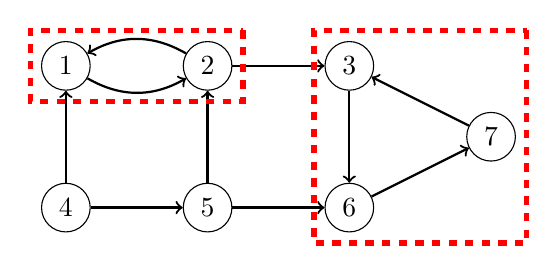
\begin{tikzpicture}[scale=0.9,label distance=-2mm]
\node[draw, circle] (1) at (-1,1) {$7$};
\node[draw, circle] (2) at (-3,2) {$3$};
\node[draw, circle] (4) at (-5,2) {$2$};
\node[draw, circle] (6) at (-7,2) {$1$};
\node[draw, circle] (3) at (-3,0) {$6$};
\node[draw, circle] (5) at (-5,0) {$5$};
\node[draw, circle] (7) at (-7,0) {$4$};

\path[draw,thick,<-] (2) -- (1);
\path[draw,thick,<-] (1) -- (3);
\path[draw,thick,<-] (3) -- (2);
\path[draw,thick,<-] (2) -- (4);
\path[draw,thick,<-] (3) -- (5);
\path[draw,thick,<-] (4) edge [bend left] (6);
\path[draw,thick,<-] (6) edge [bend left] (4);
\path[draw,thick,<-] (4) -- (5);
\path[draw,thick,<-] (5) -- (7);
\path[draw,thick,<-] (6) -- (7);

\draw [red,thick,dashed,line width=2pt] (-0.5,2.5) rectangle (-3.5,-0.5);
\draw [red,thick,dashed,line width=2pt] (-4.5,2.5) rectangle (-7.5,1.5);
%\draw [red,thick,dashed,line width=2pt] (-4.5,0.5) rectangle (-5.5,-0.5);
%\draw [red,thick,dashed,line width=2pt] (-6.5,0.5) rectangle (-7.5,-0.5);
\end{tikzpicture}
\end{center}
\end{samepage}

\begin{samepage}
Finally, the algorithm processes nodes 5 and 4
that create the remaining strongy connected components:

\begin{center}
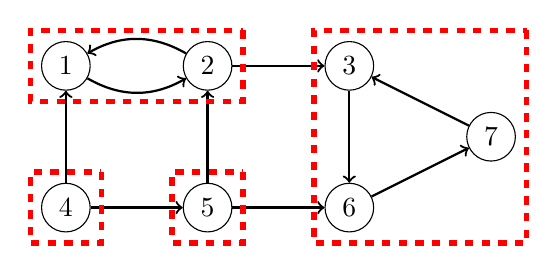
\begin{tikzpicture}[scale=0.9,label distance=-2mm]
\node[draw, circle] (1) at (-1,1) {$7$};
\node[draw, circle] (2) at (-3,2) {$3$};
\node[draw, circle] (4) at (-5,2) {$2$};
\node[draw, circle] (6) at (-7,2) {$1$};
\node[draw, circle] (3) at (-3,0) {$6$};
\node[draw, circle] (5) at (-5,0) {$5$};
\node[draw, circle] (7) at (-7,0) {$4$};

\path[draw,thick,<-] (2) -- (1);
\path[draw,thick,<-] (1) -- (3);
\path[draw,thick,<-] (3) -- (2);
\path[draw,thick,<-] (2) -- (4);
\path[draw,thick,<-] (3) -- (5);
\path[draw,thick,<-] (4) edge [bend left] (6);
\path[draw,thick,<-] (6) edge [bend left] (4);
\path[draw,thick,<-] (4) -- (5);
\path[draw,thick,<-] (5) -- (7);
\path[draw,thick,<-] (6) -- (7);

\draw [red,thick,dashed,line width=2pt] (-0.5,2.5) rectangle (-3.5,-0.5);
\draw [red,thick,dashed,line width=2pt] (-4.5,2.5) rectangle (-7.5,1.5);
\draw [red,thick,dashed,line width=2pt] (-4.5,0.5) rectangle (-5.5,-0.5);
\draw [red,thick,dashed,line width=2pt] (-6.5,0.5) rectangle (-7.5,-0.5);
\end{tikzpicture}
\end{center}
\end{samepage}

The time complexity of the algorithm is $O(n+m)$,
because the algorithm
performs two depth-first searches and
both searches take $O(n+m)$ time.

\section{2SAT problem}

\index{2SAT problem}

Strongly connectivity is also linked with the
\key{2SAT problem}.
In this problem, we are given a logical formula
\[
(a_1 \lor b_1) \land (a_2 \lor b_2) \land \cdots \land (a_m \lor b_m),
\]
where each $a_i$ and $b_i$ is either a logical variable
($x_1,x_2,\ldots,x_n$)
or a negation of a logical variable
($\lnot x_1, \lnot x_2, \ldots, \lnot x_n$).
The symbols ''$\land$'' and ''$\lor$'' denote
logical operators ''and'' and ''or''.
Our task is to assign each variable a value
so that the formula is true, or state
that this is not possible.

For example, the formula
\[
L_1 = (x_2 \lor \lnot x_1) \land
      (\lnot x_1 \lor \lnot x_2) \land
      (x_1 \lor x_3) \land
      (\lnot x_2 \lor \lnot x_3) \land
      (x_1 \lor x_4)
\]
is true when $x_1$ and $x_2$ are false
and $x_3$ and $x_4$ are true.
However, the formula
\[
L_2 = (x_1 \lor x_2) \land
      (x_1 \lor \lnot x_2) \land
      (\lnot x_1 \lor x_3) \land
      (\lnot x_1 \lor \lnot x_3)
\]
is always false, regardless of how we
choose the values of the variables.
The reason for this is that we cannot
choose a value for variable $x_1$
without creating a contradiction.
If $x_1$ is false, both $x_2$ and $\lnot x_2$
should hold which is impossible,
and if $x_1$ is true, both $x_3$ and $\lnot x_3$
should hold which is also impossible.

The 2SAT problem can be represented as a graph
whose nodes correspond to
variables $x_i$ and negations $\lnot x_i$,
and edges determine the connections
between the variables.
Each pair $(a_i \lor b_i)$ generates two edges:
$\lnot a_i \to b_i$ and $\lnot b_i \to a_i$.
This means that if $a_i$ does not hold,
$b_i$ must hold, and vice versa.

The graph for the formula $L_1$ is:
\\
\begin{center}
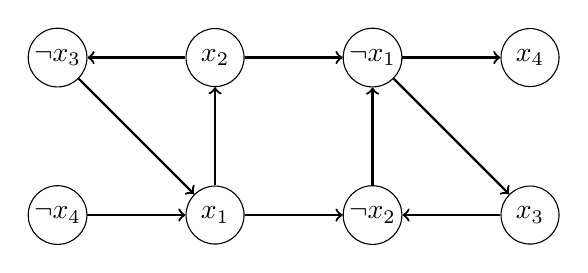
\begin{tikzpicture}[scale=1.0,minimum size=2pt]
\node[draw, circle, inner sep=1.3pt] (1) at (1,2) {$\lnot x_3$};
\node[draw, circle] (2) at (3,2) {$x_2$};
\node[draw, circle, inner sep=1.3pt] (3) at (1,0) {$\lnot x_4$};
\node[draw, circle] (4) at (3,0) {$x_1$};
\node[draw, circle, inner sep=1.3pt] (5) at (5,2) {$\lnot x_1$};
\node[draw, circle] (6) at (7,2) {$x_4$};
\node[draw, circle, inner sep=1.3pt] (7) at (5,0) {$\lnot x_2$};
\node[draw, circle] (8) at (7,0) {$x_3$};
 
\path[draw,thick,->] (1) -- (4);
\path[draw,thick,->] (4) -- (2);
\path[draw,thick,->] (2) -- (1);
\path[draw,thick,->] (3) -- (4);
\path[draw,thick,->] (2) -- (5);
\path[draw,thick,->] (4) -- (7);
\path[draw,thick,->] (5) -- (6);
\path[draw,thick,->] (5) -- (8);
\path[draw,thick,->] (8) -- (7);
\path[draw,thick,->] (7) -- (5);
\end{tikzpicture}
\end{center}
And the graph for the formula $L_2$ is:
\\
\begin{center}
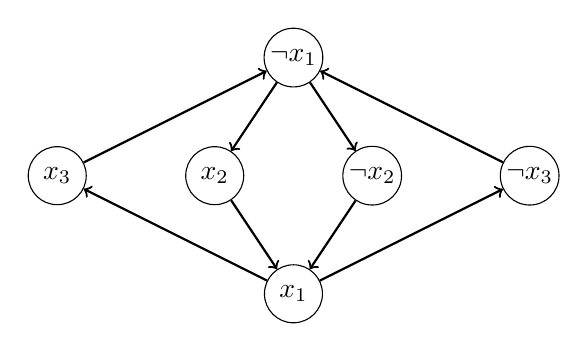
\begin{tikzpicture}[scale=1.0,minimum size=2pt]
\node[draw, circle] (1) at (1,2) {$x_3$};
\node[draw, circle] (2) at (3,2) {$x_2$};
\node[draw, circle, inner sep=1.3pt] (3) at (5,2) {$\lnot x_2$};
\node[draw, circle, inner sep=1.3pt] (4) at (7,2) {$\lnot x_3$};
\node[draw, circle, inner sep=1.3pt] (5) at (4,3.5) {$\lnot x_1$};
\node[draw, circle] (6) at (4,0.5) {$x_1$};

\path[draw,thick,->] (1) -- (5);
\path[draw,thick,->] (4) -- (5);
\path[draw,thick,->] (6) -- (1);
\path[draw,thick,->] (6) -- (4);
\path[draw,thick,->] (5) -- (2);
\path[draw,thick,->] (5) -- (3);
\path[draw,thick,->] (2) -- (6);
\path[draw,thick,->] (3) -- (6);
\end{tikzpicture}
\end{center}

The structure of the graph indicates whether
the corresponding 2SAT problem can be solved.
If there is a variable $x_i$ such that
both $x_i$ and $\lnot x_i$ belong to the
same strongly connected component,
then there are no solutions.
In this case, the graph contains
a path from $x_i$ to $\lnot x_i$,
and also a path from $\lnot x_i$ to $x_i$,
so both $x_i$ and $\lnot x_i$ should hold
which is not possible.
However, if the graph does not contain
such a variable $x_i$, then there is always a solution.

In the graph of the formula $L_1$
there are no nodes $x_i$ and $\lnot x_i$
such that both nodes 
belong to the same strongly connected component,
so there is a solution.
In the graph of the formula $L_2$
all nodes belong to the same strongly connected component,
so there are no solutions.

If a solution exists, the values for the variables
can be found by processing the nodes of the
component graph in a reverse topological sort order.
At each step, we process a component 
that does not contain edges that lead to an
unprocessed component.
If the variables in the component
have not been assigned values,
their values will be determined
according to the values in the component,
and if they already have values,
they remain unchanged.
The process continues until all variables
have been assigned a value.

The component graph for the formula $L_1$ is as follows:
\begin{center}
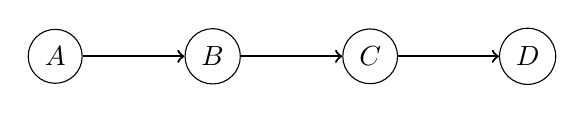
\begin{tikzpicture}[scale=1.0]
\node[draw, circle] (1) at (0,0) {$A$};
\node[draw, circle] (2) at (2,0) {$B$};
\node[draw, circle] (3) at (4,0) {$C$};
\node[draw, circle] (4) at (6,0) {$D$};

\path[draw,thick,->] (1) -- (2);
\path[draw,thick,->] (2) -- (3);
\path[draw,thick,->] (3) -- (4);
\end{tikzpicture}
\end{center}

The components are
$A = \{\lnot x_4\}$,
$B = \{x_1, x_2, \lnot x_3\}$,
$C = \{\lnot x_1, \lnot x_2, x_3\}$ and
$D = \{x_4\}$.
When constructing the solution,
we first process the component $D$
where $x_4$ becomes true.
After this, we process the component $C$
where $x_1$ and $x_2$ become false
and $x_3$ becomes true.
All variables have been assigned a value,
so the remaining components $A$ and $B$
do not change the variables.

Note that this method, works because the
structure of the graph is special.
If there are paths from node $x_i$ to node $x_j$
and from node $x_j$ to node $\lnot x_j$,
then node $x_i$ never becomes true.
The reason for this is that there is also
a path from node $\lnot x_j$ to node $\lnot x_i$,
and both $x_i$ and $x_j$ become false.

\index{3SAT problem}

A more difficult problem is the \key{3SAT problem}
where each part of the formula is of the form
$(a_i \lor b_i \lor c_i)$.
This problem is NP-hard, so no efficient algorithm
for solving the problem is known.




